\documentclass[oneside,12pt]{report}  

% the dimensions of the page
\textheight=9.25in \topmargin=-0.5in   %See note in Chapter 8 of Sample Report about "Page scaling" option in Adobe
\textwidth=6.0in
\oddsidemargin=0.3in
\evensidemargin=0.3in  % Needed to balance even and odd pages in twoside print copy


% Useful packages
\usepackage{dtklogos}
\usepackage{amsmath}
\usepackage{bm}
%\usepackage[colorlinks=true,pagebackref,linkcolor=blue]{hyperref}
\usepackage{amsfonts}
\usepackage{amsthm}
\usepackage{amsmath}
\usepackage{algorithm}
\usepackage{algorithmic}
\usepackage{graphicx, subfigure}
\usepackage{caption}
\usepackage{excludeonly}

\usepackage{listings}
\lstset{
basicstyle=\footnotesize\ttfamily,
numbers=left,
frame=bottomline,
framextopmargin=50pt,
}

\usepackage{graphicx} 

%\usepackage{doc}
%% Following sets up logic and formatting for conditional twoside copying
%\usepackage{ifthen, color, fancyvrb}
%\usepackage{nextpage}\pagestyle{plain}
%\newcommand\myclearpage{\cleartooddpage
%  [\thispagestyle{empty}]
%  }

\DeclareMathOperator*{\argmin}{arg\ min}
\DeclareMathOperator*{\sign}{sign}

% Note special alternative codes for using TWO bibliographies; see cautionary note in
\DeclareGraphicsExtensions{ps,eps,PNG,png}

% Theorem-like command definitions:
\newtheorem{theorem}{Theorem}[chapter]
\newtheorem{lemma}{Lemma}[chapter]
\newtheorem{definition}{Definition}  % Note, this italicizes everything

% Print the chapter and sections in the toc
\setcounter{tocdepth}{1}

% Specify which files to typeset for this run (note that overall pagination is preserved)
%\includeonly{chapter1, chapter2}
% Specify which files NOT to typeset for this run (note that overall pagination is preserved)
%\excludeonly{}

% Groundwork for allowing double-sided copying with blank versos
\def\prefacesection#1{
\chapter*{#1}
\addcontentsline{toc}{chapter}{#1}
}

\begin{document}


\def\thefootnote{\fnsymbol{footnote}}

\thispagestyle{empty}

% The numbers below controls the amount of space between the following sections
\def\shiftdowna{0.32in}  % Adjust for balance
\def\shiftdownb{0.22in}  % Adjust for balance

% Set up the boiler plate at the top of the page

\begin{center}
\textbf{{\large Mathematical Modeling and Consulting }}\\

%\vspace \shiftdowna
%\includegraphics[width=0.5\textwidth]{jhu.png}\\

% Home Department
\vspace \shiftdowna
\underline {Sponsor}\\ 
\vspace{5pt}
\textbf{\large National Institutes of Health} \\
\vspace\shiftdowna
\textbf{{Progress Report}}

% TITLE
\vspace \shiftdowna
\textbf{{\Large Maternal Smoking and Infant Health}}

% STUDENTS
\vspace{0.35in}
\underline {Team Members}\\
\vspace{5pt}
Yu Du, Applied Mathematics and Statistics Department\\
\texttt{ydu10@jhu.edu} \\
\vspace{10pt}
Xiaohan Yang, Applied Mathematics and Statistics Department\\
\texttt{xyang39@jhu.edu} \\
\vspace{10pt}
Hua Hua, Mechanical Engineering Department\\
\texttt{hhua1@jhu.edu}

% INSTRUCTOR
\vspace \shiftdownb
\underline {Academic Mentor} \\
\vspace{5pt}
\text{Dr.~N.~.H.~Lee}, Applied Mathematics and Statistics\\
\texttt{nhlee@jhu.edu}

% Consultants
\vspace \shiftdownb 
\underline {Consultant}\\
\vspace{5pt}
Francis Collins\\

% DATE
\vspace \shiftdowna
Date: Last Complied on \today

\end{center}

\vfill  %Fill page to force following note to bottom
\footnoterule
\noindent \small{This project was supported by National Institutes of Health.}

% Begin ABSTRACT
\ifthenelse{\boolean{@twoside}}{\myclearpage}{}
\prefacesection{Abstract}

One of the U.S. Surgeon General’s health warnings placed on the side panel of cigarette packages reads: ``Smoking by pregnant women may result in fetal injury, premature birth, and low birth weight." This project carries out statistical experiment including hypothesis tests and regression analysis to determine whether or not the above statement is true. And also we will assess what variables can influence the baby birth weight and how they can make the impact using Multiple Linear Regression Model. Then based on the given values for the predictors considered, we can make a prediction about the baby birth weight.

% Begin ACKNOWLEDGEMENTS
\ifthenelse{\boolean{@twoside}}{\myclearpage}{}
\prefacesection{Acknowledgements}

First and foremost, we would like to thank to our supervisor of this project, Dr. Lee for the valuable guidance and advice. He inspired us greatly to work in this project. His willingness to motivate us contributed tremendously to our project. We also would like to thank him for showing us some examples that related to the topic of our project. Besides, we would like to thank the authority of National Institutes of Health (NIH) for providing us with a good environment and dataset to complete this project. Finally, an honorable mention goes to our families and friends for their understandings and supports on us in completing this project. Without helps of the particular that mentioned above, we would face many difficulties while doing this.

% Table of contents, List of Figures, and List of Tables.
\ifthenelse{\boolean{@twoside}}{\myclearpage}{}
\tableofcontents

%\ifthenelse{\boolean{@twoside}}{\myclearpage}{}
%\listoffigures

%\ifthenelse{\boolean{@twoside}}{\myclearpage}{}
%\listoftables


\renewcommand{\thefootnote}{\arabic{footnote}}
\setcounter{footnote}{0}

\ifthenelse{\boolean{@twoside}}{\myclearpage}{}
\chapter{Introduction to Sponsor}\label{Introduction to Sponsor}

The National Institutes of Health (NIH), part of the U.S. Department of Health and Human Services, is the nation$'$s medical research agency---making important discoveries that improve health and save lives. Thanks in large part to NIH-funded medical research, Americans today are living longer and healthier. Life expectancy in the United States has jumped from 47 years in 1900 to 78 years as reported in 2009, and disability in people over age 65 has dropped dramatically in the past 3 decades. In recent years, nationwide rates of new diagnoses and deaths from all cancers combined have fallen significantly. 

%\include{B_TechnicalBackground}
%\include{C_ProblemStatement}

\chapter{Problem Statement}\label{Problem Statement}

One of the U.S. Surgeon General’s health warnings placed on the side panel of cigarette packages reads: ``Smoking by pregnant women may result in fetal injury, premature birth, and low birth weight." Epidemiological studies \cite{MT90} also indicate that smoking is responsible for a 150 to 250 gram reduction in birth weight and that smoking mothers are about twice as likely as nonsmoking mothers to have a low-birth-weight baby (under 2500 grams). 

\indent Since NIH is conerned about this fact, it thus sponsors the team to carry out this statistics experiment to determine the relationship between maternal smoking status and birth weight. Typically, smaller babies have lower survival rates than larger babies who are born at the same term. Therefore, birth weight is also a measure of baby health and maternal smoking status has a potential to influence the baby health. The objective NIH has in mind is to assess whether there is an impact of maternal smoking on birth weight and how if there is any impact. Futhermore, since birth weight is such an important variable, NIH is also interested in knowing what other variables influence the baby birth weight other than maternal smoking status that might include maternal height, weight, age, etc.\\
\indent In this context, the variables that concern us are birth weight, maternal smoking status, maternal weight, height, age. These variables are what we are going to consider endogenous in this project because we are going to measure the relationship among those important variables. We come up with these variables by research and also with intuition to see whether these chosen predictors have a significant impact on the response variable birth weight NIH is concerned about. Variables other than those might also have an impact on the baby birth weight, like the environment of the hospital where mothers labored and so on. But we are not going to consider those variables in this context because we mainly want to know if variables related to mothers have an impact on the baby birth weight. Those other variables are not related to mothers directly therefore those variables can be labeled as exogenous. 

%\include{D_Analysis}

%\include{E_Results}
\chapter{Analysis and Results}\label{Analysis and Results}

Data was collected from Child Health and Development Studies (CHDS)--- a comprehensive investigation of all pregnancies that occurred between 1960 and 1967 among women in the Kaiser Foundation Health Plan in the San Francisco–East Bayarea \cite{Yer71}. The data structure is listed in the following table in Figure \ref{fig:ds}.\\
\begin{figure}[htb]
    \begin{center}
        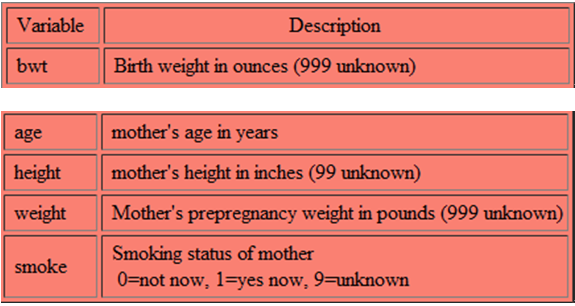
\includegraphics[width=0.75\textwidth]{DATA.png}
    \end{center}
    \caption{Data Structure}
    \label{fig:ds}
\end{figure}

First Step is importing and cleaning data.\\
\indent We import the data into R using read.csv function. There are 1236 rows and 5 columns in the original dataset:
\begin{itemize}
    \item First column: Birthweight of babies—measured in ounces
    \item Second colunm: Age of mothers—measured in years. (99 means unknown)
    \item Third column: Height of mothers—measured in inches. (99 means unknown)
    \item Fourth column: Weight of mothers—measured in pounds. (999 means unknown)
    \item Fifth column: Smoking Status of mothers—0 is nonsmoking mother, 1 is smoking mother and 9 stands for unknown situation
\end{itemize}
Then we clean the data by removing all the NA and unknown values. We index the unknown values and remove the corresponding rows and there are 1186 rows left.\\
\indent Second step is checking the basic properties of the data. From the density plots of birth weight, age, height and weight in Figure \ref{fig:densityplot}, it can be seen that all of the densities are approximately normal.
\begin{figure}[htb]
    \begin{center}
        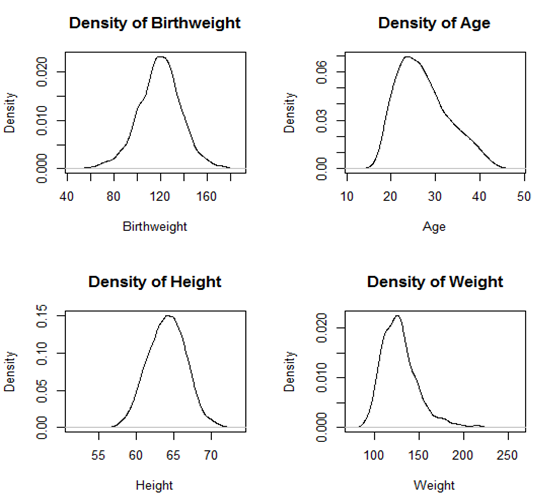
\includegraphics[width=0.85\textwidth]{densityplot.png}
    \end{center}
    \caption{Density Plots}
    \label{fig:densityplot}
\end{figure}

The range of the four variables are listed below:\\
\begin{figure}[htb]
    \begin{center}
        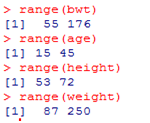
\includegraphics[width=0.237\textwidth]{range.png}
    \end{center}
    \caption{Ranges of Four Variables}
    \label{fig:range}
\end{figure}
\begin{itemize}
    \item Birthweight: minimum-55 ounces; maximum-176 ounces
    \item Age: minimum-15 years old; maximum-45 years old
    \item Height: minimum-53 inches; maximum-72 inches
    \item Weigh: minimum-87 pounds; maximum-250 pounds
\end{itemize}


Third step is splitting the data into two groups depending on mother's smoking status. One group is the birthweight for babies born to smoking mothers while the other group is the birthweight for babies born to nonsmoking mothers. There are 462 instances in smoking group while 724 instances in non-smoking group. The densities for two groups are shown in Figure \ref{fig:groupdensity}.
\begin{figure}[htb]
    \begin{center}
        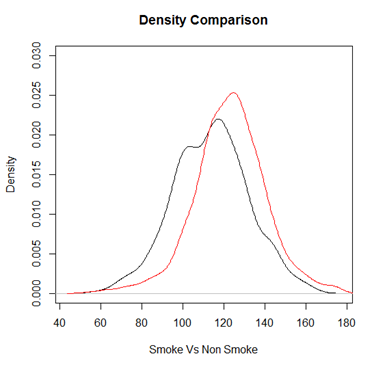
\includegraphics[width=0.66\textwidth]{groupdensity.png}
    \end{center}
    \caption{Density Comparison between Groups}
    \label{fig:groupdensity}
\end{figure}

Red line is for nonsmoking group and black line for smoking group. As is seen from this comparison of two densities, the birthweight for babies born to nonsmoking mothers tend to be larger than that for babies born to smoking mothers, which can also be supported by boxplot comparison for these two groups in Figure \ref{fig:boxplot}.
\begin{figure}[htb]
    \begin{center}
        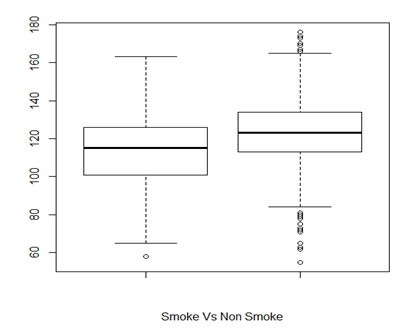
\includegraphics[width=0.75\textwidth]{boxplot.png}
    \end{center}
    \caption{Boxplots for Two Groups}
    \label{fig:boxplot}
\end{figure}

After the above preparation, we come to the fourth step, which is one of the main steps: determining whether smoking status has an impact on birth weight. We use hypothesis test and linear regression model to test it.\\
\indent First conduct two-sample hypothesis test to see if there is a difference in the birthweight of babies born to smoking mothers and born to nonsmoking mothers. To do the hypothesis test, we conduct F-test to see if we can assume equal variances for these two groups. The result is shown in Figure \ref{fig:ftest}.
\begin{figure}[htb]
    \begin{center}
        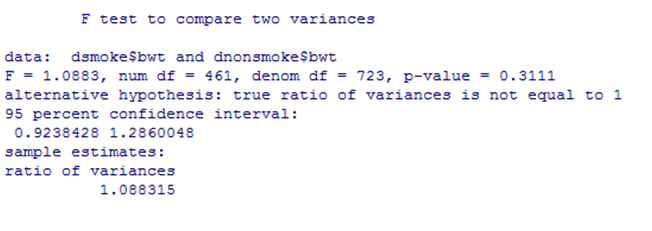
\includegraphics[width=0.96\textwidth]{ftest.png}
    \end{center}
    \caption{Results of F test}
    \label{fig:ftest}
\end{figure}
p-value is much larger than 0.05 so at the 0.05 significance level, so we do not reject the null hypothesis that two groups variances are equal.\\
\indent Therefore we assume equal variances for these two groups and move on to conduct two-sample t-test.\\
\\
\\
\\
\\
\\
\\
\\
\\
\\
\\
1)	Two Tailed T-test\\
\begin{figure}[htb]
    \begin{center}
        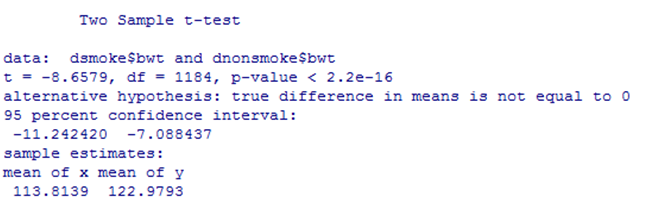
\includegraphics[width=0.95\textwidth]{twotailttest.png}
    \end{center}
    \caption{Results of Two-tailed T Test}
    \label{fig:twotailttest}
\end{figure}\\
\indent p-value is significantly small so we can conclude that the mean birthweight of babies born to smoking mothers is different from that of babies born to non-smoking mothers.\\

\noindent 2)	One Tailed T-test\\
\begin{figure}[htb]
    \begin{center}
        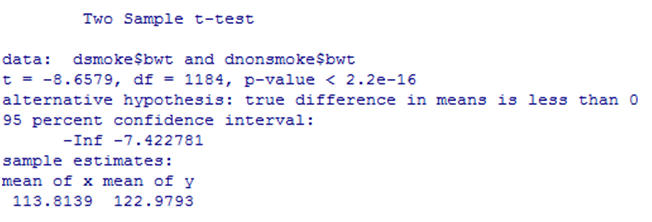
\includegraphics[width=0.95\textwidth]{onetailttest.png}
    \end{center}
    \caption{Results of One-tailed T Test}
    \label{fig:onetailttest}
\end{figure}\\
\indent p-value is significantly small so we can conclude that the mean birthweight of babies born to smoking mothers is significantly lower than that of babies born to non-smoking mothers.\\
\indent Then we conduct Linear Regression between birth weight of babies and mother’s smoking status to see if there is a difference in the birth weight of babies born to smoking mothers and born to non-smoking mothers. Result is shown in Figure \ref{fig:lrtest}.\\
\begin{figure}[htb]
    \begin{center}
        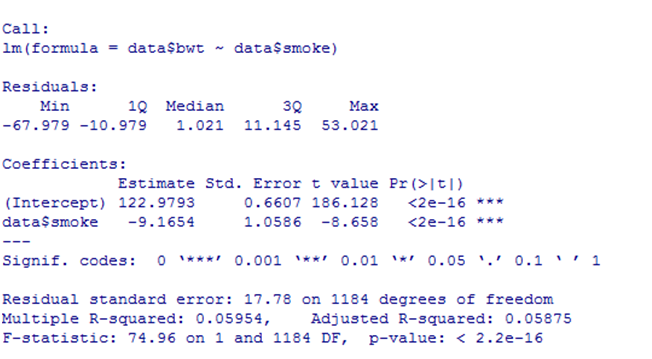
\includegraphics[width=0.855\textwidth]{lrtest.png}
    \end{center}
    \caption{Results of Linear Regression Model}
    \label{fig:lrtest}
\end{figure}
\indent Look at the variable \emph{smoke}, we can see that it is a significant variable based on the fact that its p-value is significant. And its value is -9.1654, which is negative, so smoking mothers have a negative impact on baby birth weights, the same as what we concluded above.\\
\indent Our last step is to check whether other variables maternal height, weight and age also have impact on birth weigh, to build a multiple linear regression model containing the influential variables and to use the model to predict birth weight.\\
\indent First we do multiple linear regression for the response variable baby birth weight against the predictors mother’s age, height, weight as well as mother’s smoking status in order to predict baby birth weight given the values for the predictors. The result in R is in Figure \ref{fig:mlr4}.\\
\begin{figure}[htb]
    \begin{center}
        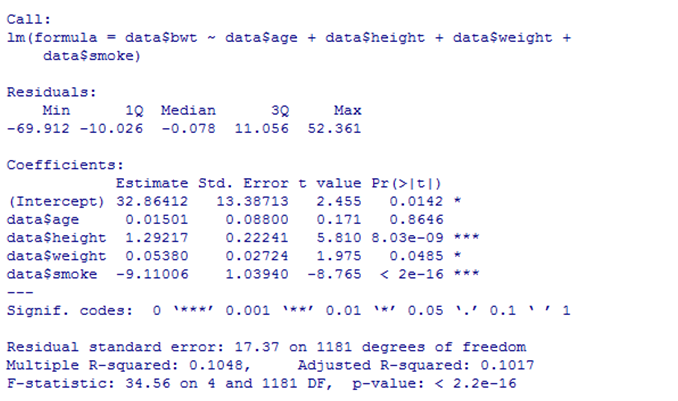
\includegraphics[width=0.863\textwidth]{mlr4.png}
    \end{center}
    \caption{Multiple Linear Regression Containing All Variables}
    \label{fig:mlr4}
\end{figure}\\
\indent All the predictors are significant except mother’s age whose p-value is much larger than 0.05. This indicates that mother’s age is not a good indicator for baby birth weight. We can also use AIC score to conclude this. See Figure \ref{fig:aic}.
\begin{figure}[htb]
    \begin{center}
        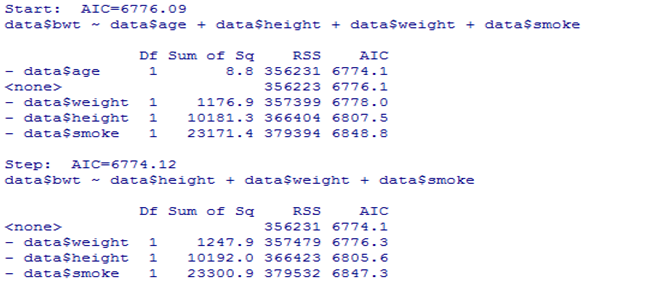
\includegraphics[width=\textwidth]{aic.png}
    \end{center}
    \caption{AIC Scores}
    \label{fig:aic}
\end{figure}\\
\indent When we remove the variable mother’s age, we can derive a lower AIC which is better. So we reestablish our model with mother’s age being removed. The model is shown in Figure \ref{fig:mlr3}.
\begin{figure}[htb]
    \begin{center}
        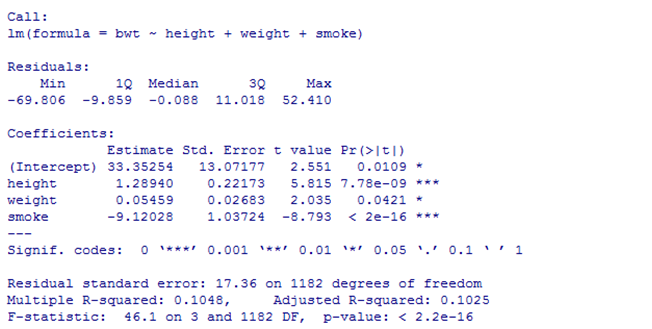
\includegraphics[width=\textwidth]{mlr3.png}
    \end{center}
    \caption{Multiple Linear Regression Without Age}
    \label{fig:mlr3}
\end{figure}\\
\indent Now all the predictors are significant with p-values all much larger than 0.05.\\
\indent To do further test of the model, it can be seen from the residual plot in Figure \ref{fig:residualplot} that there is no specific pattern for residuals and they are distributed randomly around the zero line. So the assumptions about residuals can be considered met.\\
\begin{figure}[htb]
    \begin{center}
        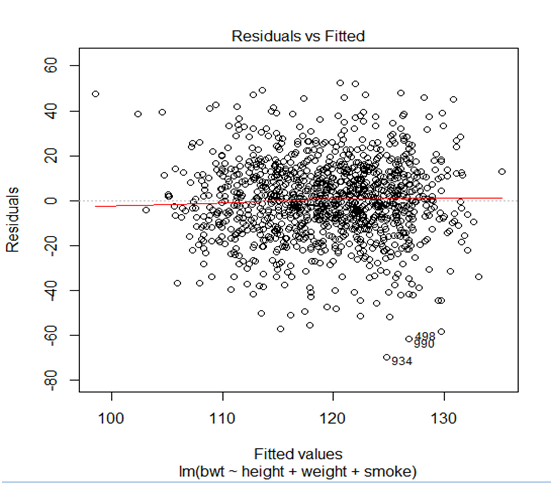
\includegraphics[width=0.9\textwidth]{residualplot.png}
    \end{center}
    \caption{Residual Plot}
    \label{fig:residualplot}
\end{figure}\\
So we come to our final model:
\[
\begin{split}
     Birth~Weight=&~33.35254 - 9.12028 (Maternal~Smoking~Status)\\ 
                  &+ 1.28940 (Maternal~Height) + 0.05459(Maternal~Weight)
\end{split}
\]
\indent Then we can predict birth weight using the model above with values of predictors given. Suppose we are interested in knowing the birth weight of the baby born to a mother whose height is 60 inches, weight is 150 pounds and smoked during her pregnancy. Prediction Interval is $[75.59127, 143.9787]$ as shown below:\\
\begin{figure}[htb]
    \begin{center}
        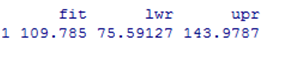
\includegraphics[width=0.4\textwidth]{predict1.png}
    \end{center}
    \caption{Prediction Interval for Smoking Mother}
    \label{predict1}
\end{figure}\\
\indent Suppose we are interested in knowing the birth weight of the baby born to a mother whose height is 60 inches, weight is 150 pounds and did not smoke during her pregnancy. Prediction Interval is $[84.73556, 153.0749]$ as shown below:\\
\begin{figure}[htb]
    \begin{center}
        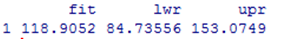
\includegraphics[width=0.4\textwidth]{predict2.png}
    \end{center}
    \caption{Prediction Interval for Nonsmoking Mother}
    \label{predict2}
\end{figure}\\
\indent From these two intervals we can also see that babies born to nonsmoking mothers tend to have larger weight than those born to smoking mothers.


%\include{F_Conclusion}
\chapter{Conclusion}\label{Conclusion}

Our team has two tasks for this project as stated in \emph{Problem Statement} part: determing whether there is a relationship between maternal smoking status and birth weight, and discussing whether maternal height, weight and age influence the baby birth weight.\\
\indent For the first task, we used several ways to test whether maternal smoking affects the birth weight. We first plotted the line graph and boxplot for distributions of the birth weight in two groups and compared the graphs to get an intuitive concept. Then we did two-sided and one-sided hypothesis tests to obtain more convincing evidence. At last, we used linear regression model to check the significance level of the independent variable maternal smoking status on dependent variable birth weight.\\
\indent All the methods in \emph{Analysis and Results} part lead to the conclusion that maternal smoking status has an influence on the birth weight of the children. If a mother smokes, the birth weight of her child is expected to be smaller than that of a child whose mother does not smoke.\\
\indent For the second task, we built a linear regression model of birth weight on all the four independent variables: maternal height, weight, age and smoking status, and checked the significance level of each independent variable. From these procedures, we observed that maternal height, weight and smoking status impact birth weight significantly while maternal age has insignificant effect. So we ruled out the variable maternal age and found that the model containing the other three independent variables was the best.\\
\indent In conclusion, among the four independent variables we study, maternal height and weight have significant positive influence on the baby birth weigh, that is, the taller or heavier a mother is, the heavier the child is expected to be. Smoking has significant negative impact on baby birth weight. It leads to an expectation of less weight. Age has insignificant influence on baby birth weight. We can simply ignore it.\\
\indent With respect to future research, two main things need to be done. On one hand, data need further clean. By checking the data, we found some very influential ones. These data may be outliers and influence the results and conclusions we just got. We will decide how we should deal with them. We may do some adjustments to them or delete them. On the other hand, one of the deliverables of our project is a software that produces the prediction interval of baby birth weight given the values of the predictors as the input. So we need to develop the software based on our final regression model.


%\include{chapter1}
%\include{chapter2}
%\include{chapter3}
%\include{chapter4}
%\include{chapter5}
%\include{chapter6}


\appendix
\ifthenelse{\boolean{@twoside}}{\myclearpage}{}

%\chapter{Lemmas}\label{Lemma}

%\chapter{Glossary}\label{Glossary}

%\vspace{12pt} 

%\vspace{8pt}
%\noindent {\bf Ascending node}. The point where the satellite crosses through
%the equatorial plane in a northerly direction. 



\ifthenelse{\boolean{@twoside}}{\myclearpage}{}
\chapter{Abbreviations}\label{Abbreviations}


\noindent NIH.  National Institutes of Health, part of the U.S. Department of Health and Human Services

\vspace{5pt}

\noindent CHDS. Child Health and Development Studies, a comprehensive investigation of all pregnancies that occurred between 1960 and 1967 among women in the Kaiser Foundation Health Plan in the San Francisco–East Bayarea

\vspace{5pt}



\ifthenelse{\boolean{@twoside}}{\myclearpage}{}
\chapter{R Codes}\label{R Codes}

{\bf Import data:}
\begin{lstlisting}
data=read.csv("birthweight.csv")
dim(data)
attach(data)
\end{lstlisting}

\noindent{\bf Clean data:}
\begin{lstlisting}
index1=which(weight=="999")
index2=which(height=="99")
index3=which(smoke==9)
index4=which(age==99)
index=c(index1,index2,index3,index4)
length(index)
data=data[-index,]
dim(data)
attach(data)
\end{lstlisting}

\noindent{\bf Plot the distribution of variables:}
\begin{lstlisting}
par(mfrow=c(2,2))
plot(density(bwt),main="Density of Birthweight",xlab="Birthweight")
plot(density(age),main="Density of Age",xlab="Age")
plot(density(height),main="Density of Height",xlab="Height")
plot(density(weight),main="Density of Weight",xlab="Weight")
\end{lstlisting}

\noindent{\bf Split data into two groups depending on mother's smoking status:}
\begin{lstlisting}
smoke1=which(smoke==1)
dsmoke=data[smoke1,]
dsmoke
dnonsmoke=data[-smoke1,]
dnonsmoke
dim(dsmoke)[1]
dim(dnonsmoke)[1]
\end{lstlisting}

\noindent{\bf Compare the distribution of two groups:}
\begin{lstlisting}
plot(density(dsmoke$bwt),ylim=c(0,0.03),xlab="Smoke Vs Non Smoke")
lines(density(dnonsmoke$bwt),add=T)
boxplot(dsmoke$bwt,dnonsmoke$bwt,xlab="Smoke Vs Non Smoke")
\end{lstlisting}

\noindent{\bf Hypothesis test on means of birthweight of two groups:}
\begin{lstlisting}
var.test(dsmoke$bwt,dnonsmoke$bwt)
t.test(dsmoke$bwt,dnonsmoke$bwt,var.equal=TRUE,paired=FALSE)
t.test(dsmoke$bwt,dnonsmoke$bwt,var.equal=TRUE,paired=FALSE,alternative="less")
\end{lstlisting}

\noindent{\bf Linear regressing of birthweight on smoking status:}
\begin{lstlisting}
fit1=lm(data$bwt~data$smoke)
summary(fit1)
\end{lstlisting}

\noindent{\bf Linear regression on all variables:}
\begin{lstlisting}
fit2=lm(data$bwt~data$age+data$height+data$weight+data$smoke)
summary(fit2)
st=step(fit2)
install.packages("car")
library(car)
vif(fit2)
plot(vif(fit2))
attach(data)
fit3=lm(bwt~height+weight+smoke)
summary(fit3)
plot(fit3)
pred1=data.frame(height=60,weight=150,smoke=1)
pred2=data.frame(height=60,weight=150,smoke=0)
predict(fit3,pred1,interval="predict")
predict(fit3,pred2,interval="predict")
\end{lstlisting}


%\endinput

% Add your bibliography to Contents
\ifthenelse{\boolean{@twoside}}{\myclearpage}{\newpage}
\addtocontents {toc}{\protect \contentsline {chapter}{REFERENCES}{}}
\addcontentsline{toc}{chapter}{Selected Bibliography Including Cited Works}  

% Bibliography must come last.
\bibliographystyle{plain}
\renewcommand\bibname{Selected Bibliography Including Cited Works}
\nocite{*}  % List ALL references in your references, not just the ones cited in the text.
% This scheme automatically alphabetizes the Bibliography.
\bibliography{reference}
\end{document}
